\newpage
\section{Sviluppatore}
Lo sviluppatore è in grado di eseguire tutte le operazioni disponibili al cliente e in aggiunta può inserire API nel market e trasferire il guadagno proveniente dalla vendita nel suo saldo Paypal.
Uno sviluppatore deve inserire, se non fatto al momento della registrazione i seguenti dati obbligatori:
	
\begin{itemize}
	\item Descrizione personale;
	\item Immagine personale;
	\item Email PayPal.
\end{itemize}


\subsection{API registrate}
Lo sviluppatore all'interno della sua area personale può visualizzare le API registrate e le loro caratteristiche principali.

\label{API registrate}
\begin{figure}[H]
	\centering
	\fbox{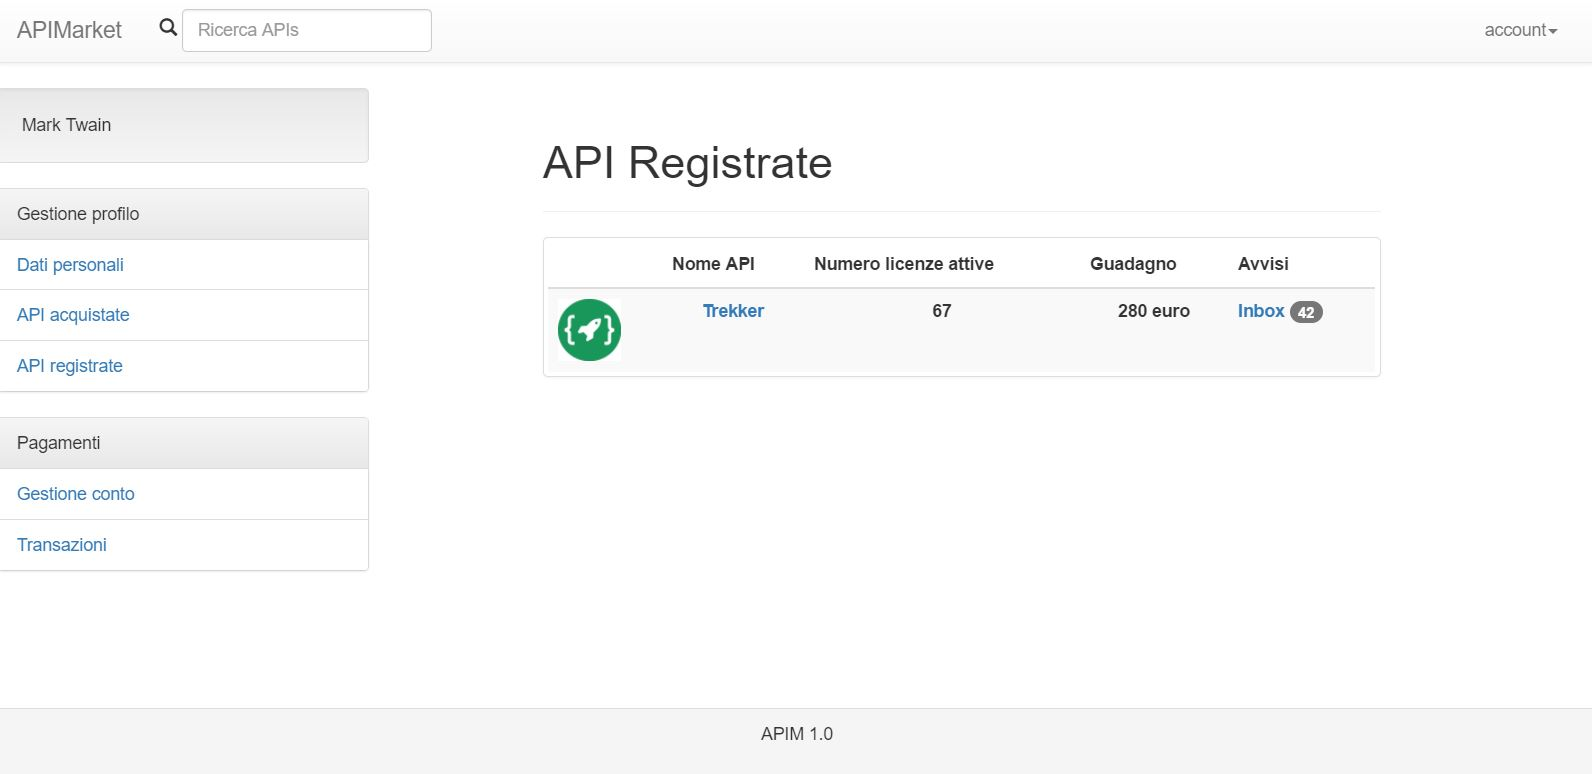
\includegraphics[scale=0.31]{img/APIM_apiRegistrate.JPG}}
	\caption{API registrate}
\end{figure}

\subsection{Registrazione API}

L'utente abilitato alla vendita (Sviluppatore) può  registrare le proprie API per la vendita nell'apposita pagina accessibile dal profilo utente. La schermata per la registrazione di nuove API appare come mostrato nell'immagine sottostante.

\label{Registrazione API}
\begin{figure}[H]
	\centering
	\fbox{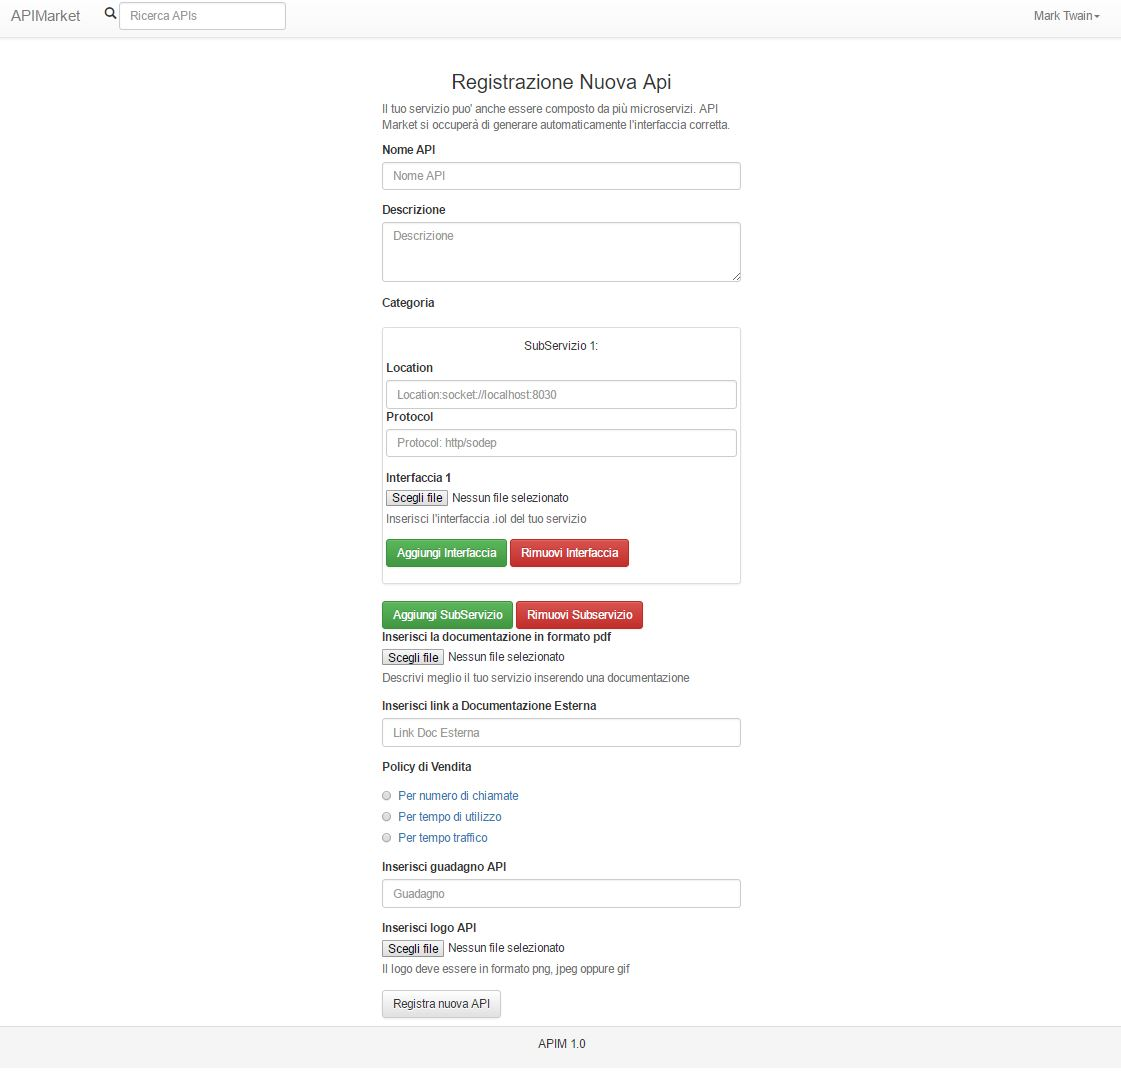
\includegraphics[scale=0.31]{img/APIM_nuovaApi.JPG}}
	\caption{Registrazione API}
\end{figure}

All'interno, l'utente dovrà specificare obbligatoriamente i seguenti dati per permettere l'inserimento del proprio prodotto nella piattaforma

\begin{itemize}
	\item Nome dell'API;
	\item Breve descrizione;
	\item Tags che identificano le categorie a cui appartiene;
	\item L'URI/Posizione del servizio;
	\item Il protocollo di comunicazione utilizzato;
	\item I file che caratterizzano l'interfaccia;
	\item Posizione, protocollo e interfaccia di eventuali sottoservizi correlati (opzionale);
	\item Documentazione PDF o link esterno;
	\item Il guadagno desiderato e la policy scelta;
	\item Il logo del prodotto.
\end{itemize}

Qualora i campi inseriti fossero corretti, il sistema segnala che la procedura è andata a buon fine.

\subsection{Pagamenti}
Lo sviluppatore accumula il guadagno della vendita delle sue API, nel suo conto personale; esso può decidere di trasferire il ricavato sul suo conto Paypal, collegato all'indirizzo email inserito nel suo profilo.
L'operazione è possibile tramite il pulsante "NOME PULSANTE" per poi completare la transazione sul sito PAYPAL???

IMMAGINE CONTO PERSONALE
